\documentclass{ctexart}
\usepackage[a4paper,scale=0.8,centering]{geometry}
\usepackage{graphicx,xcolor}
\usepackage{listings}
\lstset{
    columns=fixed,       
    numbers=left,                                        % 在左侧显示行号
    frame=none,                                          % 不显示背景边框
    backgroundcolor=\color[RGB]{245,245,244},            % 设定背景颜色
    keywordstyle=\color[RGB]{40,40,255},                 % 设定关键字颜色
    numberstyle=\footnotesize\color{darkgray},           % 设定行号格式
    commentstyle=\it\color[RGB]{0,96,96},                % 设置代码注释的格式
    stringstyle=\rmfamily\slshape\color[RGB]{128,0,0},   % 设置字符串格式
    showstringspaces=false,                              % 不显示字符串中的空格
}

\title{绘制Bezier曲线}
\author{St Maxwell}
\date{\today}
\begin{document}
\maketitle
\section{Bezier曲线}
Bezier曲线是常用于计算机图形学等相关领域的一种参数曲线。

一条Bezier曲线是由一组控制点定义的,其中第一个点和最后一个点总是曲线的起点和终点,中间的控制点通常不在曲线上。根据点的数量不同,有不同阶数的Bezier曲线。

\noindent
\textbf{线性Bezier曲线}

给定点$\mathbf{P}_0$、$\mathbf{P}_1$,线性Bezier曲线只是一条两点之间的直线。这条线由下式给出:
\[
\mathbf{B}(t) = (1 - t)\mathbf{P}_0 + t\mathbf{P}_1,\quad t \in [0, 1]
\]

\noindent
\textbf{二次方Bezier曲线}

二次方Bezier曲线的路径由给定点$\mathbf{P}_0$、$\mathbf{P}_1$、$\mathbf{P}_2$的函数$\mathbf{B}(t)$追踪:
\[
\mathbf{B}(t) = (1 - t)^2\mathbf{P}_0 + 2t(1-t)\mathbf{P}_1 + t^2\mathbf{P}_2,\quad t \in [0, 1]
\]

\noindent
\textbf{三次方Bezier曲线}

$\mathbf{P}_0$、$\mathbf{P}_1$、$\mathbf{P}_2$、$\mathbf{P}_3$四个点在平面或在三维空间中定义了三次方Bezier曲线。曲线起始于$\mathbf{P}_0$走向$\mathbf{P}_1$,并从$\mathbf{P}_2$的方向来到$\mathbf{P}_3$。
\[
\mathbf{B}(t) = (1 - t)^3\mathbf{P}_0 + 3t(1-t)^2\mathbf{P}_1 + 3t^2(1-t)\mathbf{P}_2 + t^3\mathbf{P}_3,\quad t \in [0, 1]
\]

\begin{figure}[htbp]
    \centering
    \includegraphics[width=25em]{Bezier_curve.pdf}
    \caption{四个控制点的三次方Bezier曲线}
    \label{fig:plot1}
\end{figure}

\section{Fortran实现}
使用Fortran实现可获得三种平面Bezier曲线的离散点的功能。代码中的\texttt{BezierCurve}子程序接受的参数有离散点的个数\texttt{npts},用于控制曲线的光滑程度。\texttt{P0}到\texttt{P3}是控制点坐标,其中\texttt{P2}和\texttt{P3}是可选参数。只输入两个点的坐标,输出的就是线性Bezier曲线;输入三个点的坐标,得到二次方Bezier曲线;全部都输入则是三次方Bezier曲线。\texttt{BzPts}是输出的曲线离散点的二维数组。

{\setmainfont{Consolas}                          % 设置代码字体                   
\begin{lstlisting}[language=Fortran]
module global
  implicit none
  contains
  subroutine BezierCurve(BzPts,npts,P0,P1,P2,P3)
    implicit none
    real(kind=8),intent(in) :: P0(2),P1(2)
    real(kind=8),intent(in),optional :: P2(2),P3(2)
    integer,intent(in) :: npts
    real(kind=8),intent(out) :: BzPts(:,:)
    real(kind=8) :: step
    real(kind=8) :: t, t2, t3, tp, tp2, tp3
    integer :: i
    logical :: bl1, bl2 ! determine the existence of P2, P3
    
    bl1 = present(P2)
    bl2 = present(P3)
    step = 1.0D0 / npts
    t = 0.0D0
    if (bl1 .and. bl2) then
      ! cubic bezier curve when four points passed
      BzPts(npts+1,:) = P3
      do i = 1, npts
        tp = (1.0D0 - t)
        tp2 = tp * tp
        tp3 = tp2 * tp
        t2 = t * t
        t3 = t2 * t
        BzPts(i,:) = P0*tp3 + 3.0D0*P1*t*tp2 + 3.0D0*P2*tp*t2 + P3*t3
        t = t + step
      end do
    else if (bl1 .or. bl2) then
      ! quadratic bezier curve when three points passed
      BzPts(npts+1,:) = P2
      do i = 1, npts
        tp = (1.0D0 - t)
        tp2 = tp * tp
        t2 = t * t
        BzPts(i,:) = P0*tp2 + 2.0D0*P1*t*tp + P2*t2
        t = t + step
      end do
    else
      ! linear bezier curve when two points passed
      BzPts(npts+1,:) = P1
      do i = 1, npts
        tp = (1.0D0 - t)
        BzPts(i,:) = P0*tp + P1*t
        t = t + step
      end do
    end if
    
  end subroutine
end module
program main
  use global
  implicit none
  real(kind=8) :: P0(2) = (/ 0.0D0, 0.0D0 /)
  real(kind=8) :: P1(2) = (/ 1.0D0, 1.0D0 /)
  real(kind=8) :: P2(2) = (/ 2.0D0,-1.0D0 /)
  real(kind=8) :: P3(2) = (/ 3.0D0, 0.0D0 /)
  integer :: n = 50
  real(kind=8),allocatable :: B(:,:)
  integer :: i
  
  allocate(B(n+1,2))
  call BezierCurve(B,n,P0,P1)
  write(*,*) "Linear Bezier Curve"
  do i = 1, size(B,1)
    write(*,"(F6.3,'  ',F6.3)") B(i,:)
  end do
  call BezierCurve(B,n,P0,P1,P2)
  write(*,*) "Quadratic Bezier Curve"
  do i = 1, size(B,1)
    write(*,"(F6.3,'  ',F6.3)") B(i,:)
  end do
  call BezierCurve(B,n,P0,P1,P2,P3)
  write(*,*) "Cubic Bezier Curve"
  do i = 1, size(B,1)
    write(*,"(F6.3,'  ',F6.3)") B(i,:)
  end do
  
end program
\end{lstlisting}}

选择$(0,0)$、$(1,1)$、$(2,-1)$、$(3,0)$四个点,计算三种Bezier曲线的离散点。将输出的坐标点在Origin中绘制成图。

\begin{figure}[htbp]
    \centering
    \includegraphics[width=22em]{graph.pdf}
    \caption{线性、二次方、三次方Bezier曲线}
    \label{fig:plot2}
\end{figure}

\section{绘制字母}
用以上的Fortran代码计算得到的点绘制较为复杂的图形比较困难,因此使用Mathematica的\\ \texttt{BezierCurve}函数进行绘图。

首先要获取字体字形上的端点坐标,并选择合适的控制点。

\begin{figure}[htbp]
    \centering
    \includegraphics[width=20em]{W.png}
    \caption{字母W}
    \label{fig:plot3}
\end{figure}

用以下Mathematica代码绘制图形:
{\setmainfont{Consolas}                          % 设置代码字体                   
\begin{lstlisting}[language=Mathematica,morekeywords={BezierCurve}]
Graphics[{
    BezierCurve[{{0,0},{0,-3.4}}],
    BezierCurve[{{0,-3.4},{5,-3.4},{13,-7},{15,-13}}],
    BezierCurve[{{15,-13},{57,-130}}],
    BezierCurve[{{57,-130},{60.3,-130}}],
    BezierCurve[{{60.3,-130},{89.1,-48.8}}],
    BezierCurve[{{89.1,-48.8},{118,-130}}],
    BezierCurve[{{118,-130},{122,-130}}],
    BezierCurve[{{122,-130},{161,-17}}],
    BezierCurve[{{161,-17},{165,-7},{168,-3.4},{177.2,-3.4}}],
    BezierCurve[{{177.2,-3.4},{177.2,0}}],
    BezierCurve[{{177.2,0},{139.2,0}}],
    BezierCurve[{{139.2,0},{139.2,-3.4}}],
    BezierCurve[{{139.2,-3.4},{150,-3.8},{157,-10},{150,-25}}],
    BezierCurve[{{150,-25},{125,-97.7}}],
    BezierCurve[{{125,-97.7},{100,-27}}],
    BezierCurve[{{100,-27},{93,-10},{95,-3.4},{109.9,-3.4}}],
    BezierCurve[{{109.9,-3.4},{109.9,0}}],
    BezierCurve[{{109.9,0},{60.5,0}}],
    BezierCurve[{{60.5,0},{60.5,-3.4}}],
    BezierCurve[{{60.5,-3.4},{70,-3.4},{75,-10},{79,-20}}],
    BezierCurve[{{79,-20},{85,-37}}],
    BezierCurve[{{85,-37},{63.8,-97.7}}],
    BezierCurve[{{63.8,-97.7},{35,-14}}],
    BezierCurve[{{35,-14},{33,-7},{42,-3.4},{47,-3.4}}],
    BezierCurve[{{47,-3.4},{47,0}}],
    BezierCurve[{{47,0},{0,0}}]
}]                                                           
\end{lstlisting}}

\begin{figure}[htbp]
    \centering
    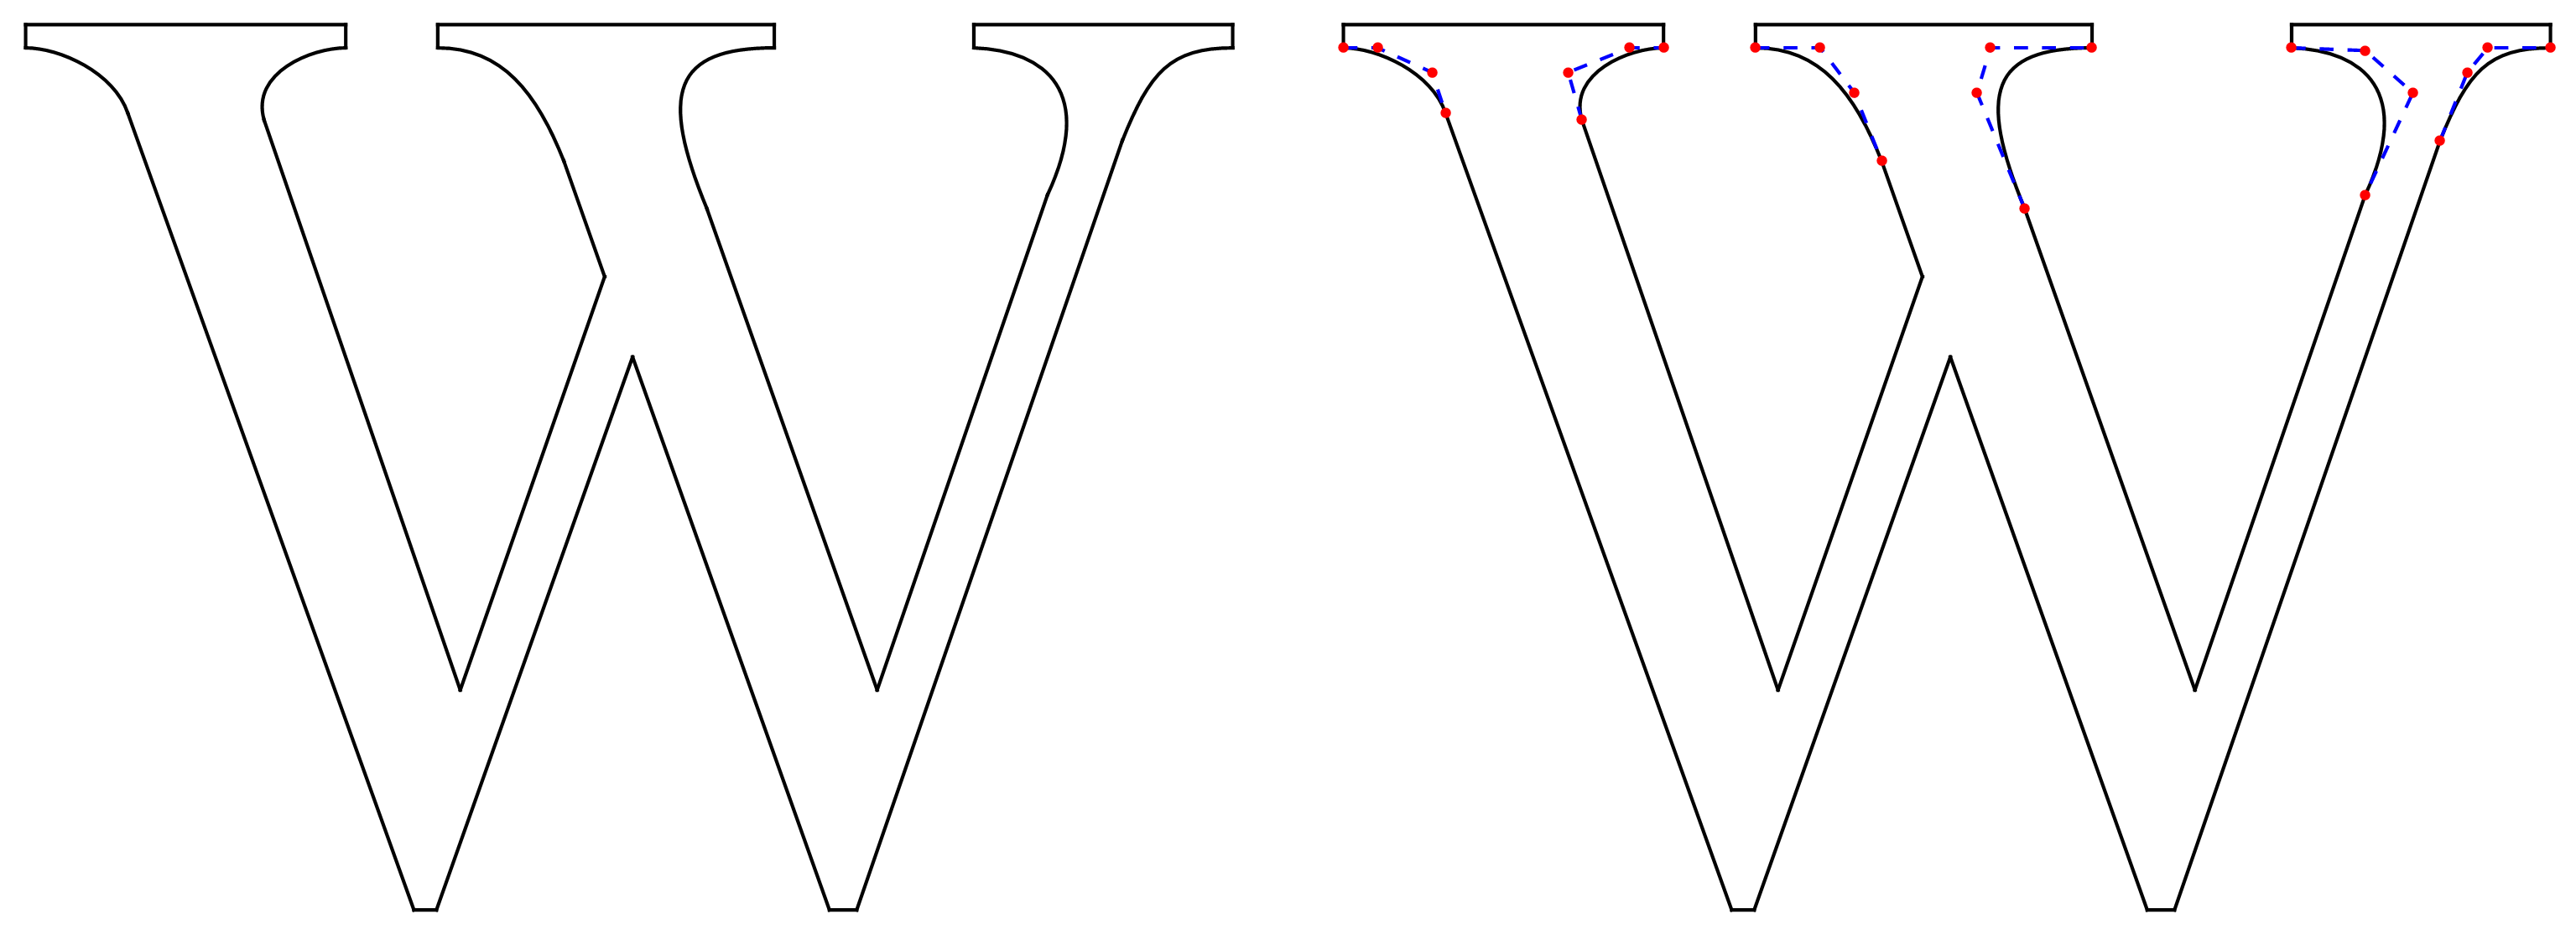
\includegraphics[width=25em]{WW.png}
    \caption{用Bezier曲线绘制的Times New Roman字体的字母W}
    \label{fig:plot4}
\end{figure}

基于相同的步骤,绘制出字母B、C、D。

\begin{figure}[htbp]
    \centering
    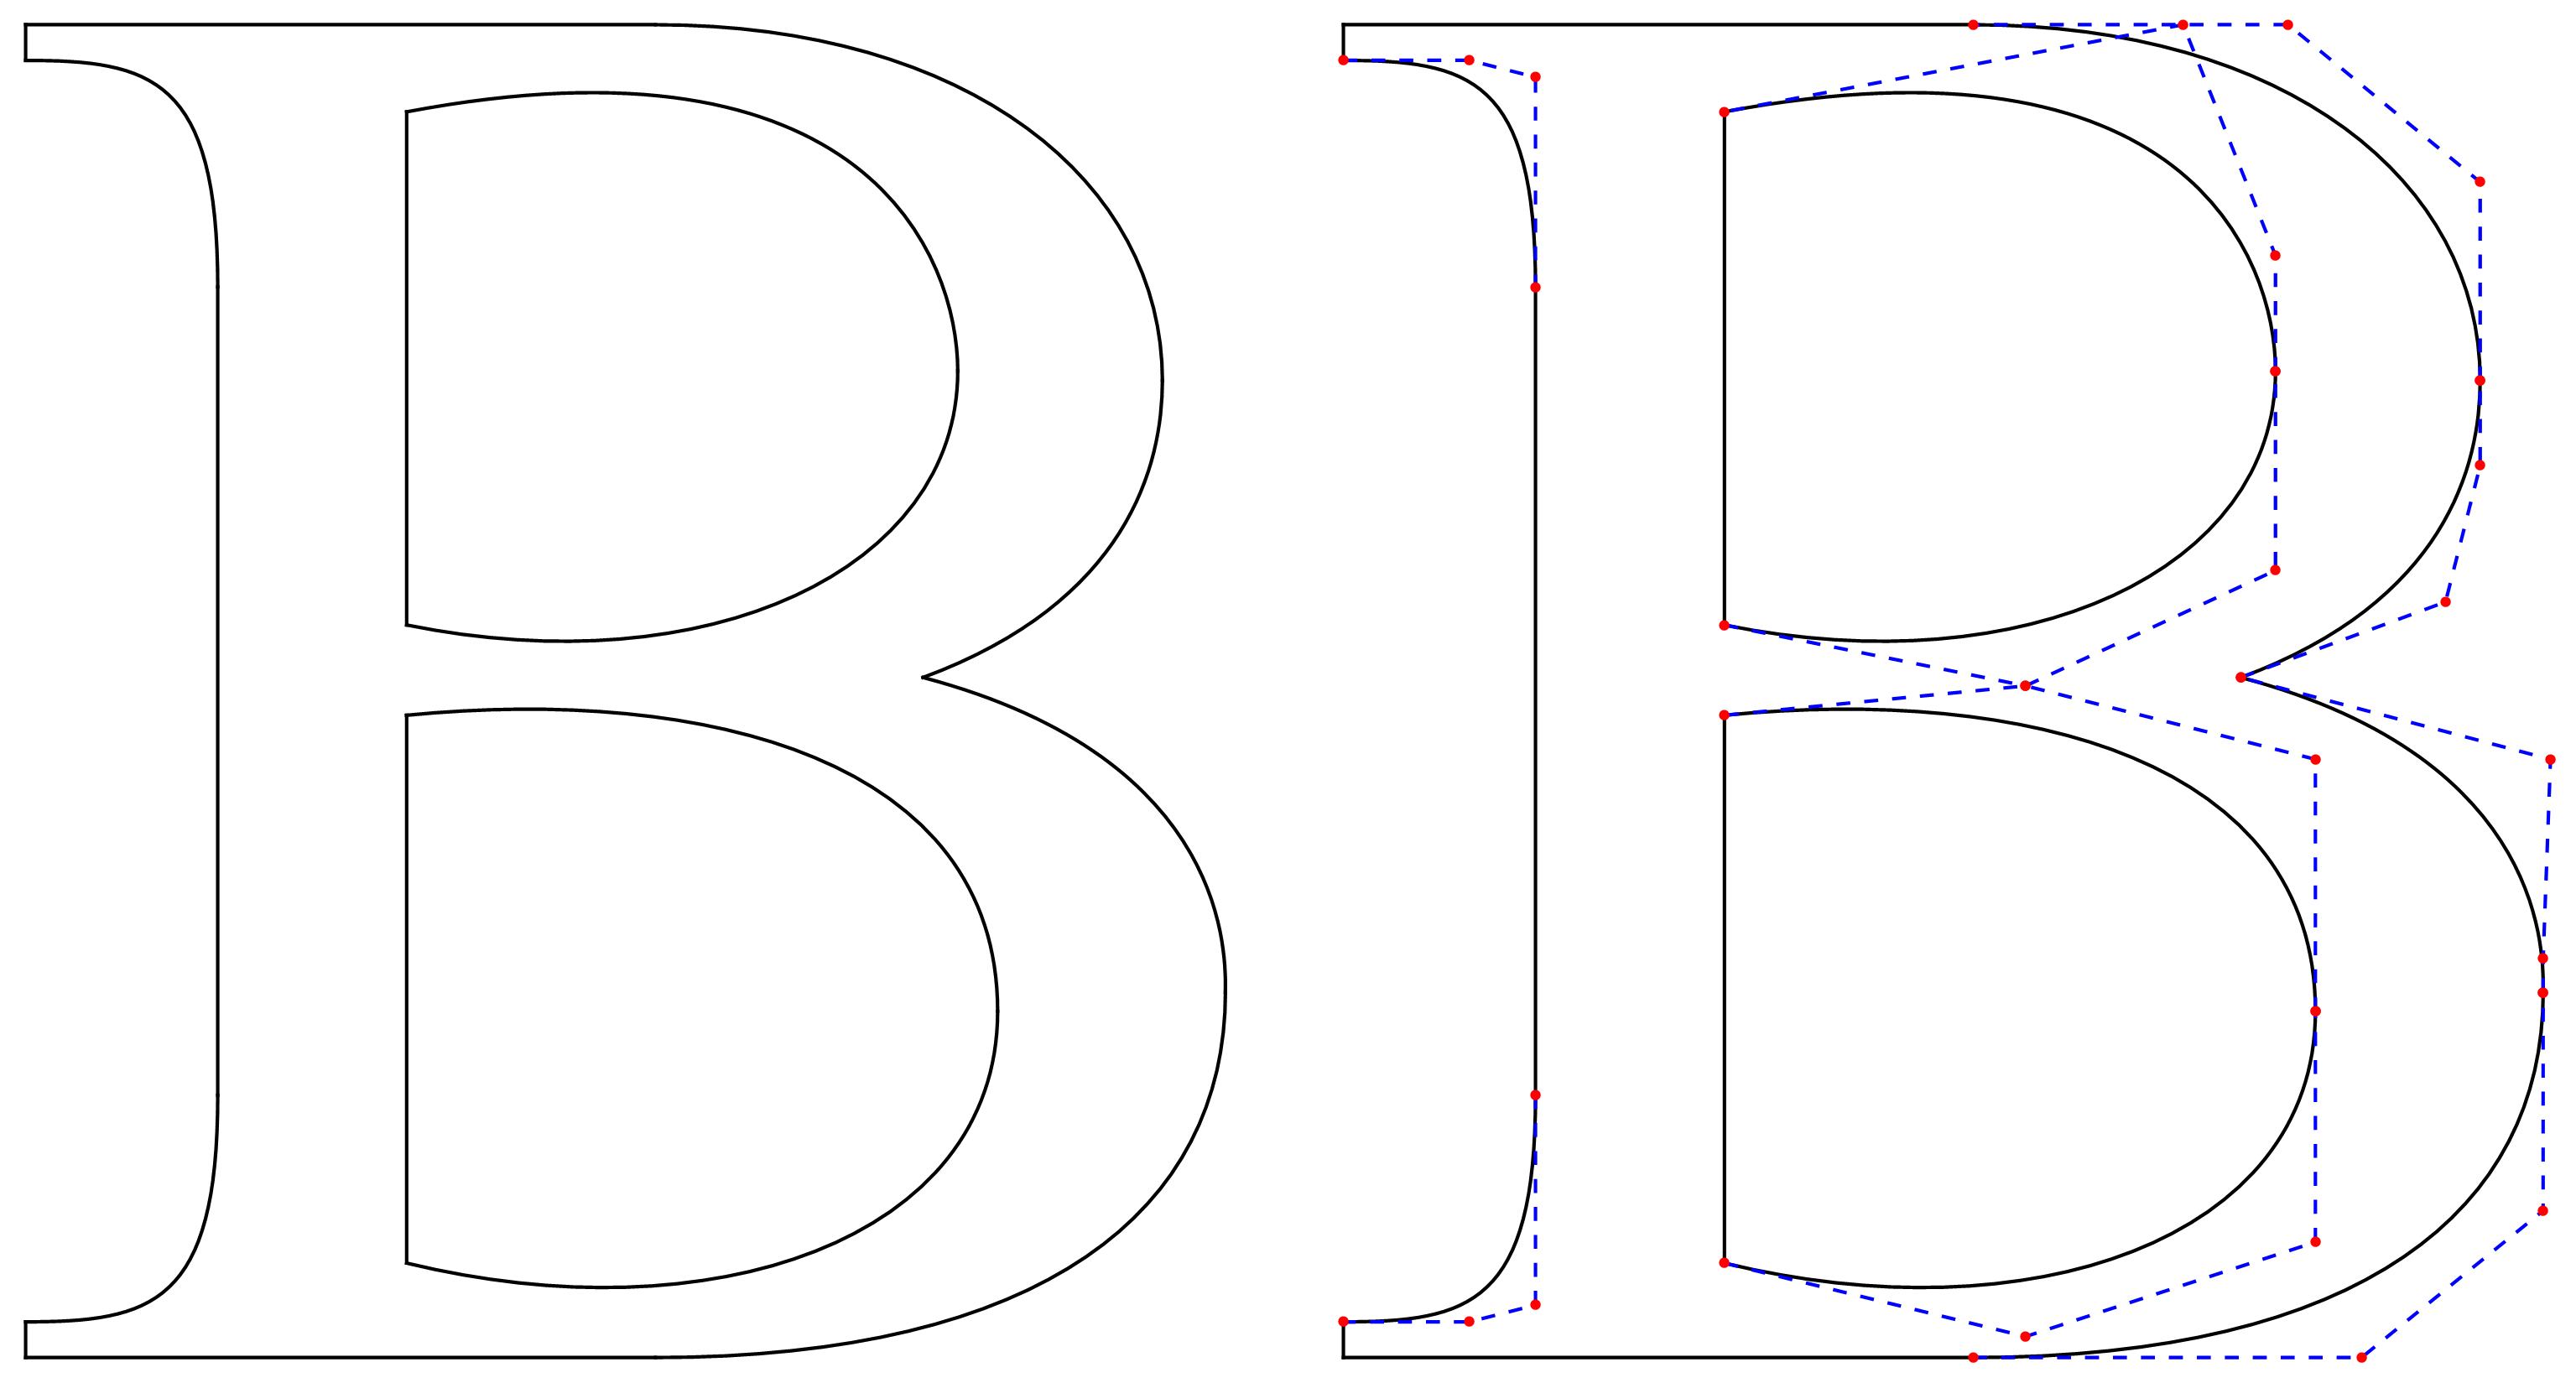
\includegraphics[width=25em]{BB.png}
    \caption{用Bezier曲线绘制的Times New Roman字体的字母B}
    \label{fig:plot5}
\end{figure}

\begin{figure}[htbp]
    \centering
    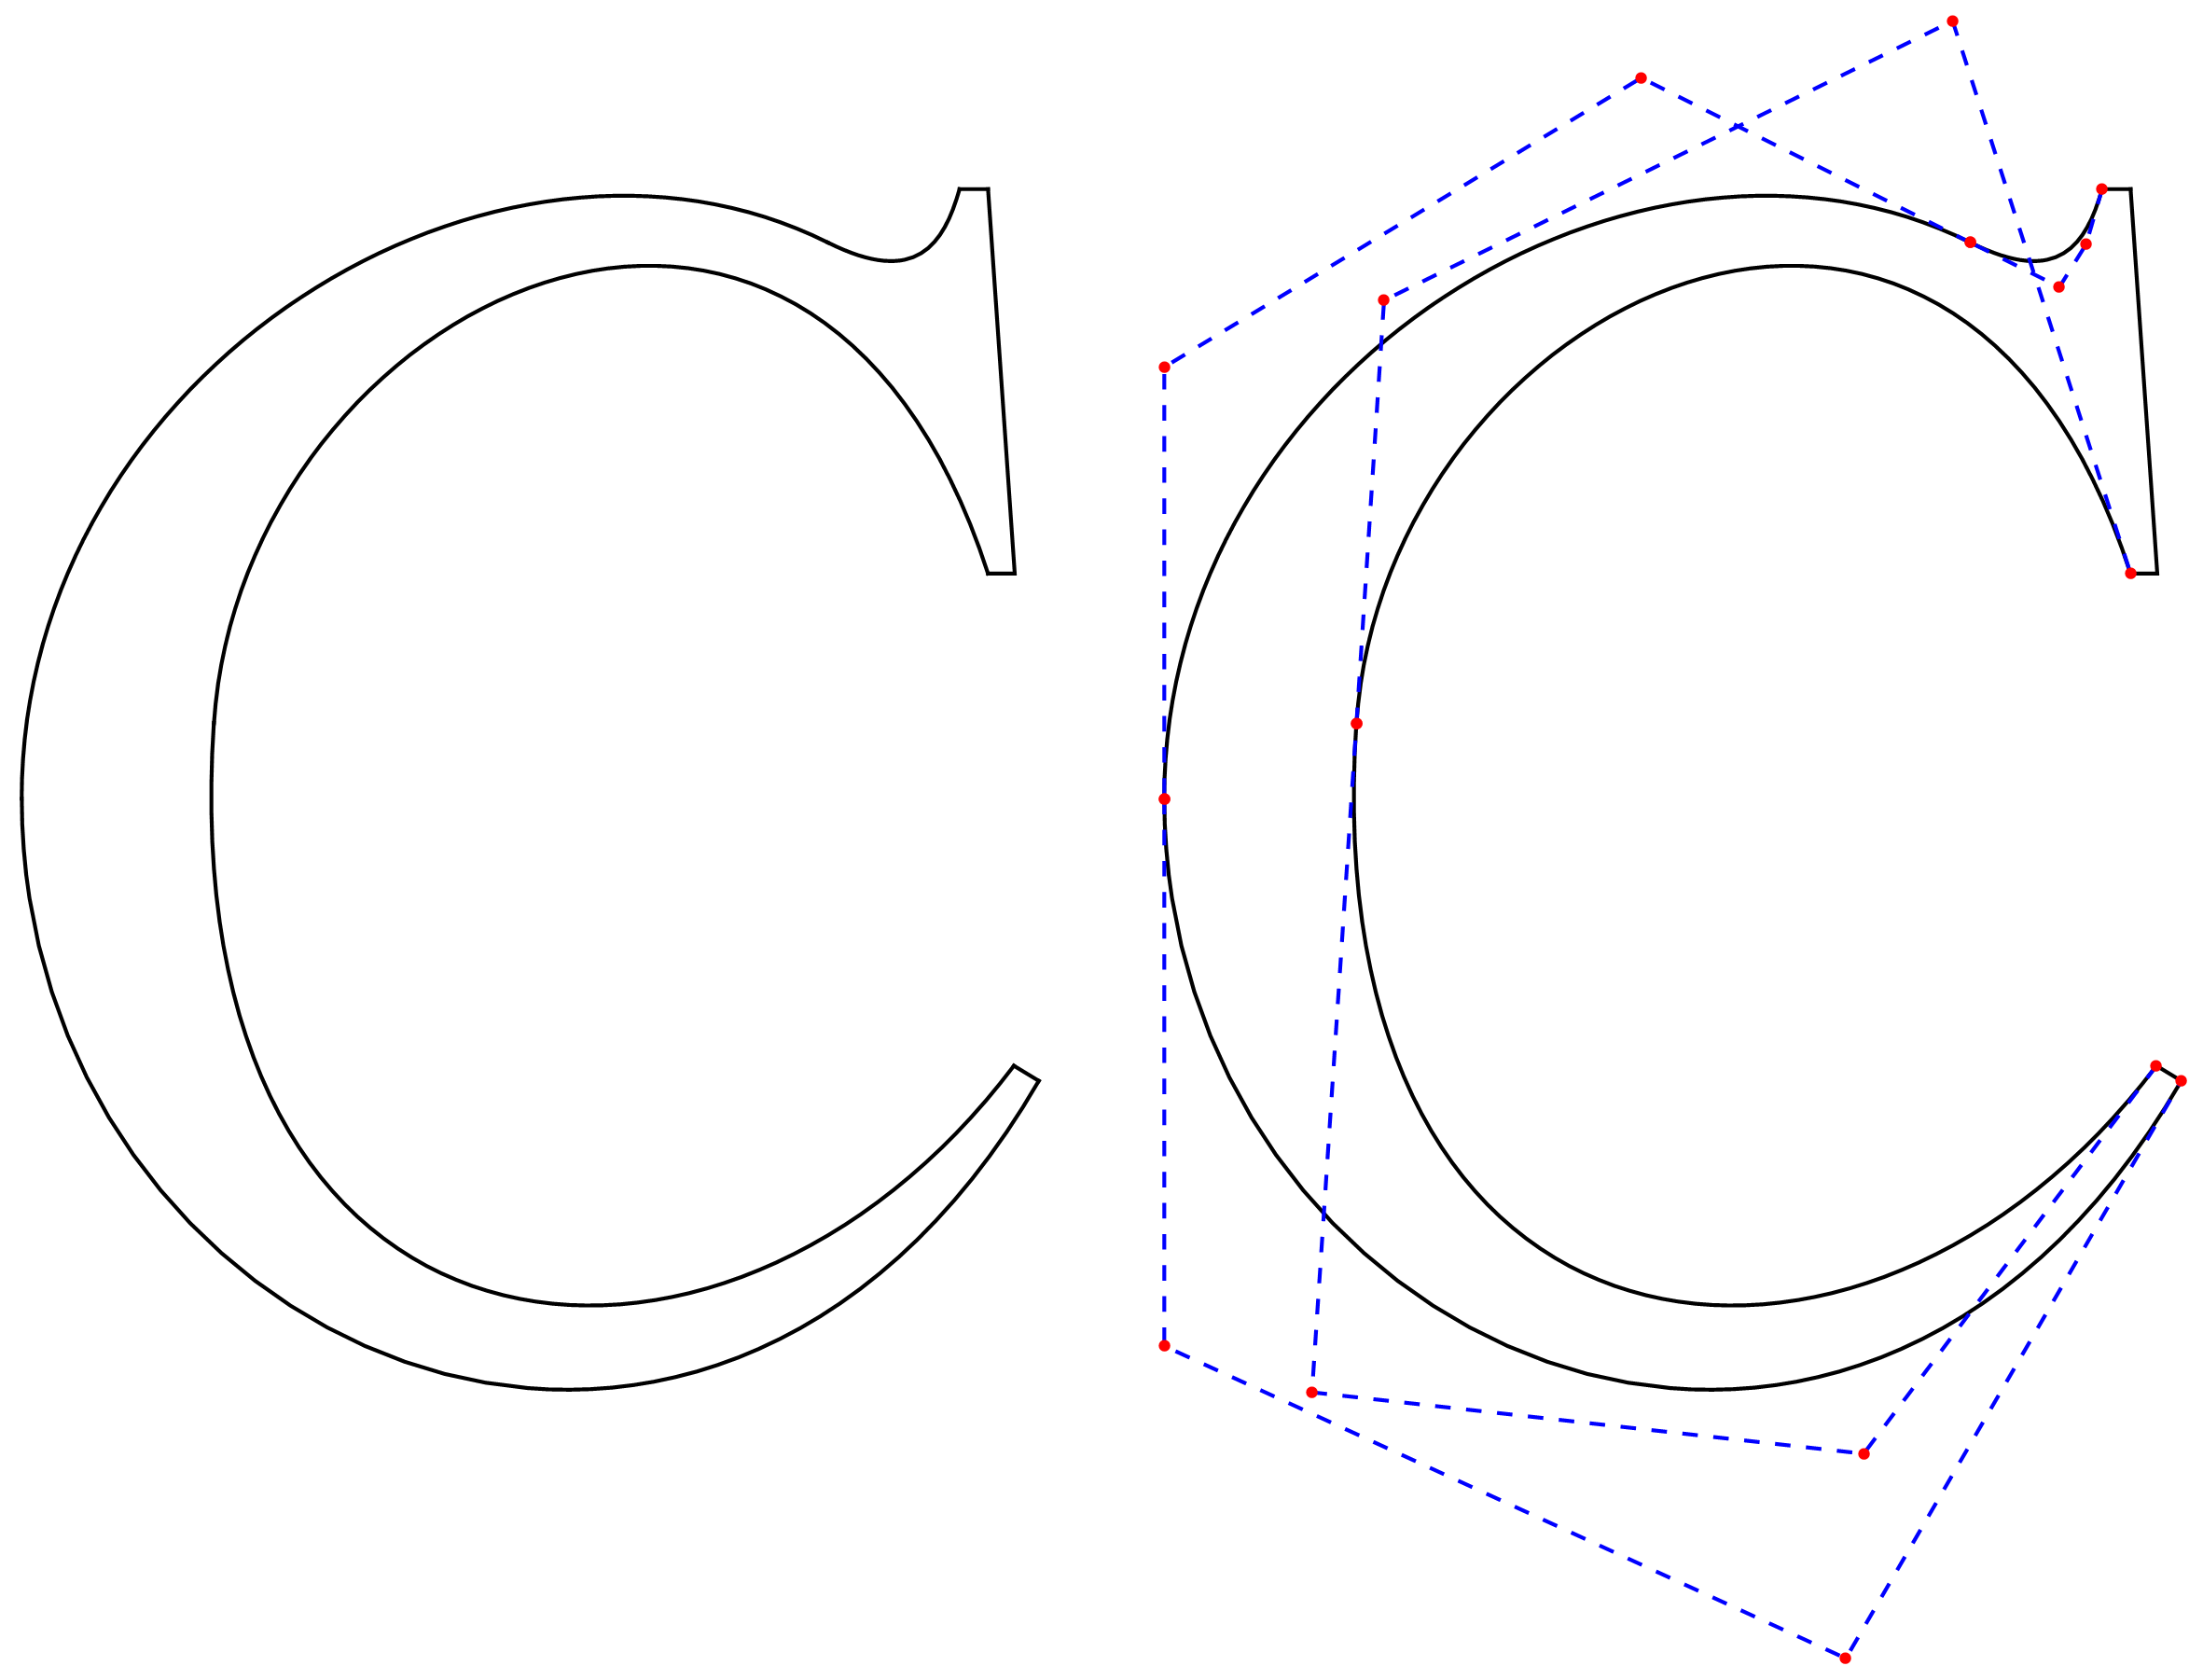
\includegraphics[width=25em]{CC.png}
    \caption{用Bezier曲线绘制的Times New Roman字体的字母C}
    \label{fig:plot6}
\end{figure}

\begin{figure}[htbp]
    \centering
    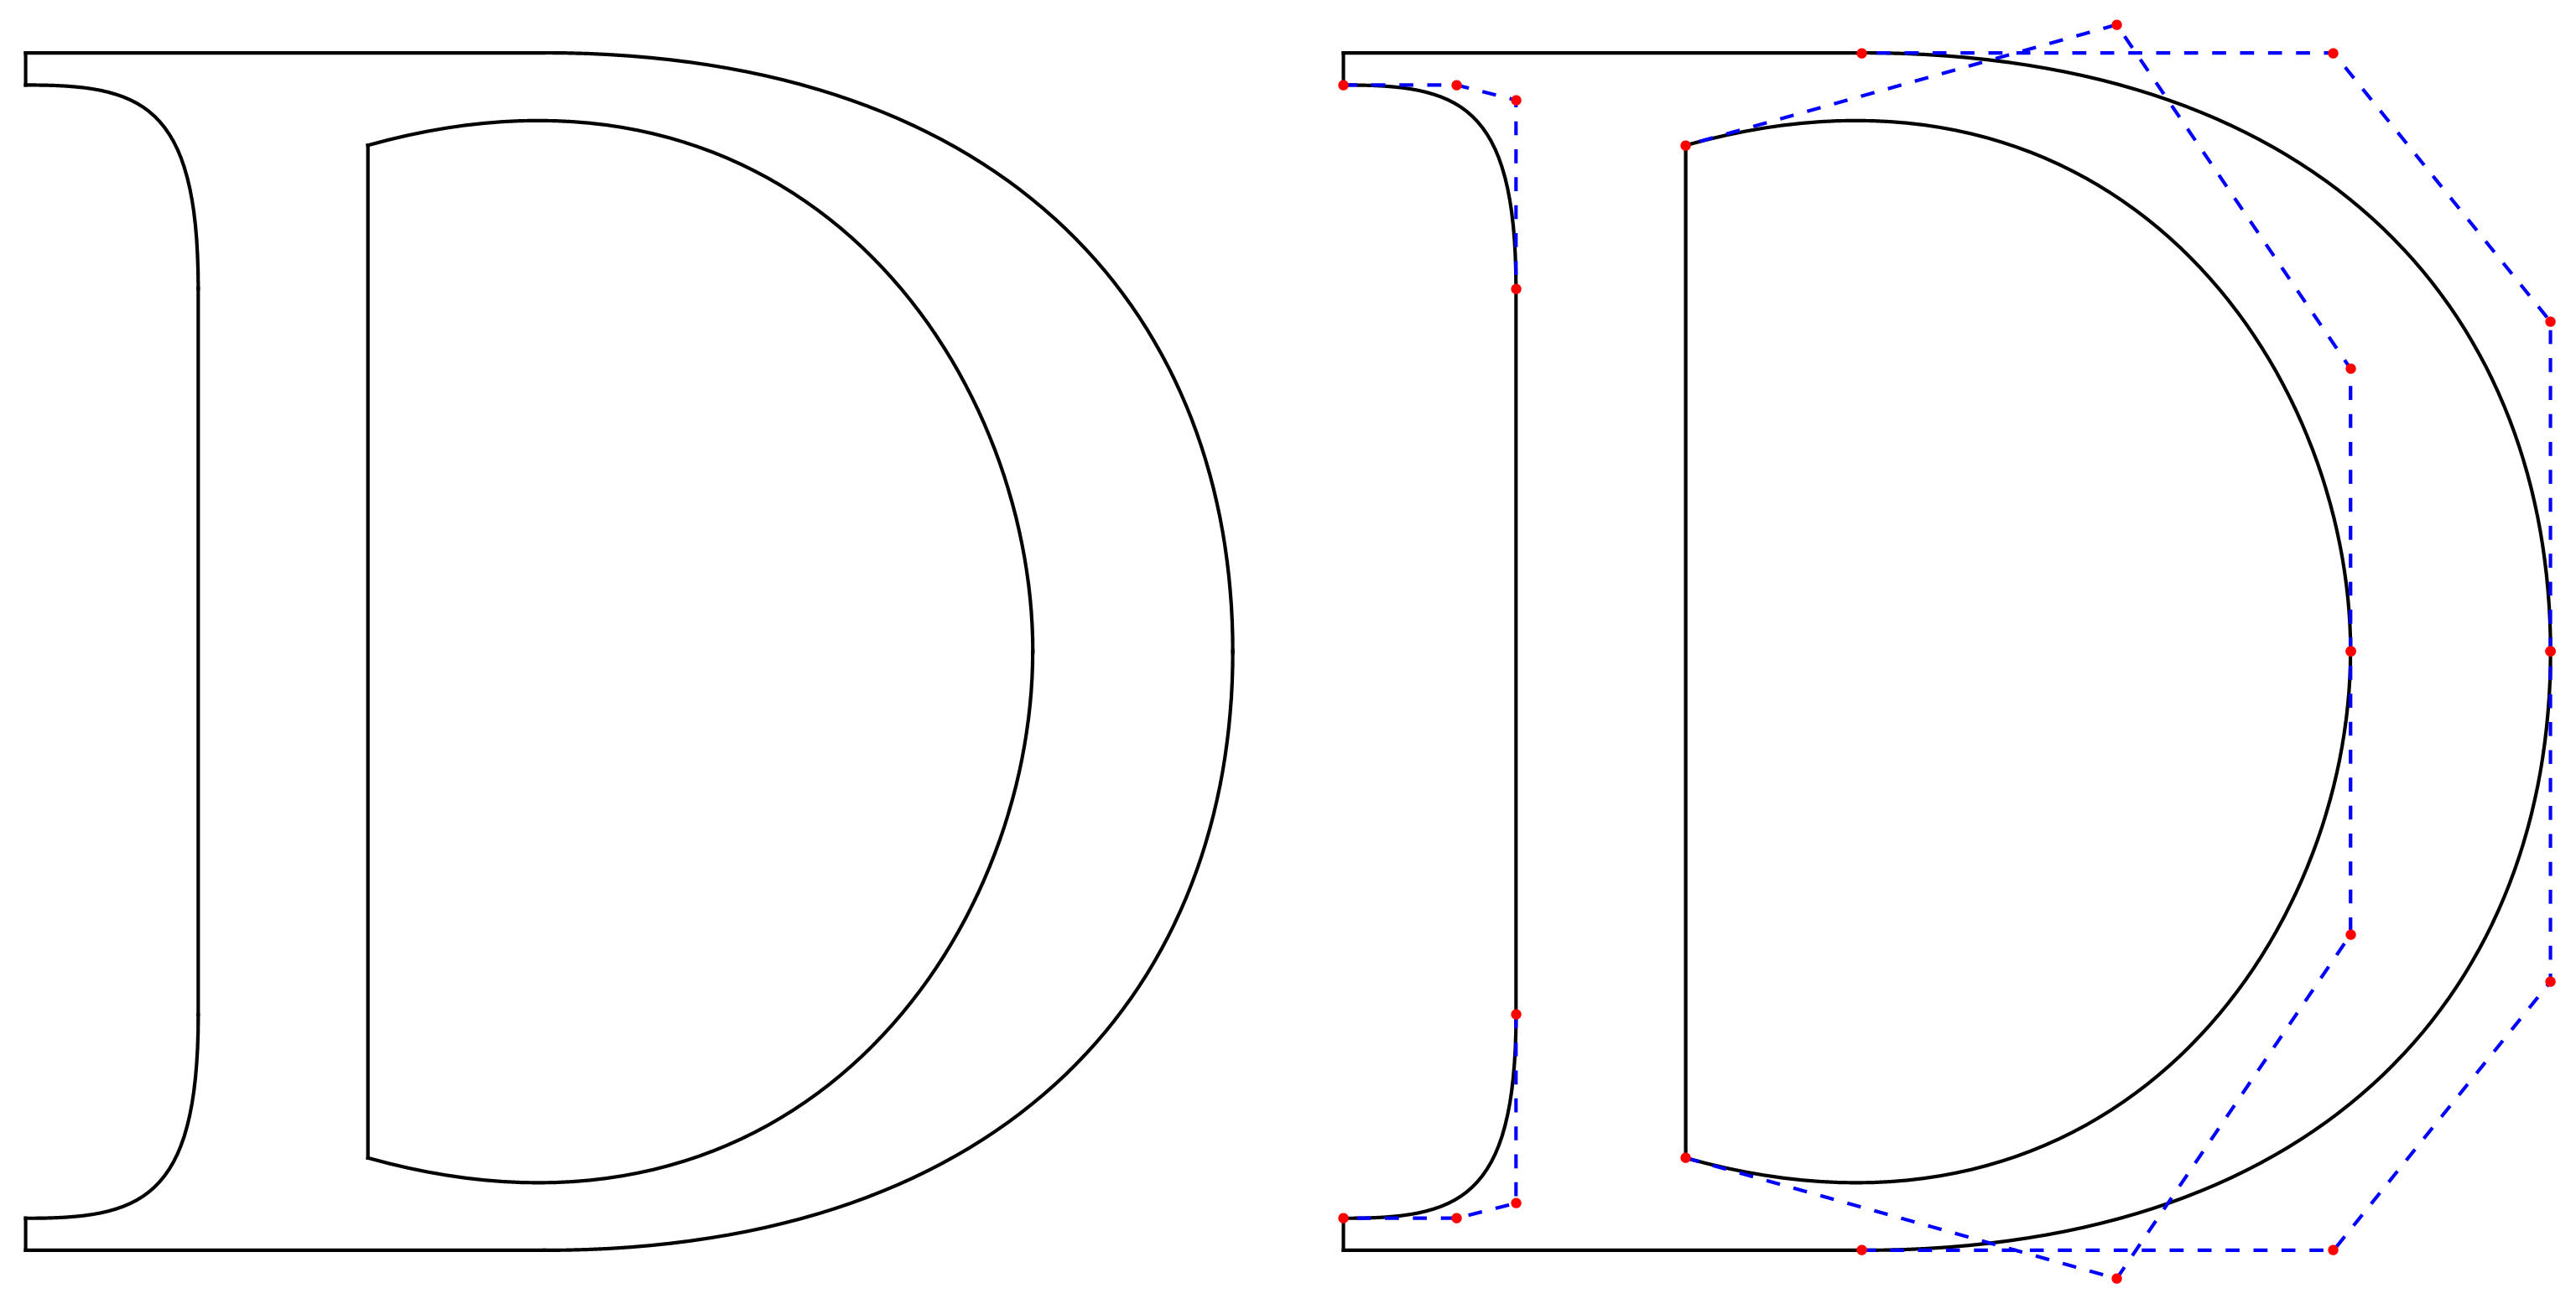
\includegraphics[width=25em]{DD.png}
    \caption{用Bezier曲线绘制的Times New Roman字体的字母D}
    \label{fig:plot7}
\end{figure}

\end{document}